\documentclass[11pt,a4paper]{report} 

% Für doppelseitigen Ausdruck (nur bei > 60 Seiten sinnvoll)
% \usepackage{ifthen}
% \setboolean{@twoside}{true}
% \setboolean{@openright}{true} 

% Deutsch
\usepackage[german]{babel} % deutsch und deutsche Rechtschreibung
\usepackage[utf8]{inputenc} % Unicode Text 
\usepackage[T1]{fontenc} % Umlaute und deutsches Trennen
\usepackage{textcomp} % Euro
\usepackage[hyphens]{url}
% statt immer Ab\-schluss\-ar\-beit zu schreiben
% einfach hier sammeln mit -. 
\hyphenation{Ab-schluss-ar-beit}
% Vorsicht bei Umlauten und Bindestrichen
\hyphenation{Ver-st\"ar-ker-aus-gang}
 % eigene Hyphenations, die für das Dokument gelten
\usepackage{amssymb} % Symbole
\usepackage{emptypage} % Wirklich leer bei leeren Seiten

%% Fonts, je ein kompletter Satz an Optionen

% Times New Roman, gewohnter Font, ok tt und serifenlos
%\usepackage{mathptmx} 
%\usepackage[scaled=.95]{helvet}
%\usepackage{courier}

% Palatino mit guten Fonts für tt und serifenlos
\usepackage{mathpazo} % Palatino, mal was anderes
\usepackage[scaled=.95]{helvet}
\usepackage{courier}

% New Century Schoolbook sieht auch nett aus (macht auch tt und serifenlos)
%\usepackage{newcent}

% Oder default serifenlos mit Helvetica 
% ich kann es nicht mehr sehen ...
%\renewcommand{\familydefault}{\sfdefault}

% ein bisschen eine bessere Verteilung der Buchstaben...
\usepackage{microtype}

% Bilder und Listings
\usepackage{graphicx} % wir wollen Bilder einfügen
\usepackage{subfig} % Teilbilder
\usepackage{wrapfig} % vielleicht doch besser vermeiden
\usepackage{listings} % schöne Quellcode-Listings
% ein paar Einstellungen für akzeptable Listings
\lstset{basicstyle=\ttfamily, columns=[l]flexible, mathescape=true, showstringspaces=false, numbers=left, numberstyle=\tiny}
\lstset{language=python} % und nur schöne Programmiersprachen ;-)
% und eine eigene Umgebung für Listings
\usepackage{float}
\newfloat{listing}{htbp}{scl}[chapter]
\floatname{listing}{Listing}

% Seitenlayout
\usepackage[paper=a4paper,width=14.2cm,left=36mm,height=22cm]{geometry}
\usepackage{setspace}
\linespread{1.15}
\setlength{\parskip}{0.5em}
\setlength{\parindent}{0em} % im Deutschen Einrückung nicht üblich, leider

% Seitenmarkierungen 
\newcommand{\phv}{\fontfamily{phv}\fontseries{m}\fontsize{9}{11}\selectfont}
\usepackage{fancyhdr} % Schickere Header und Footer
\pagestyle{fancy}
\renewcommand{\chaptermark}[1]{\markboth{#1}{}}
%\fancyhead[L]{\phv \leftmark}
\fancyhead[RE,LO]{\phv \nouppercase{\leftmark}}
\fancyhead[LE,RO]{\phv \thepage}
% Unten besser auf alles Verzichten
%\fancyfoot[L]{\textsf{\small \kurztitel}}
\fancyfoot[C]{\ } % keine Seitenzahl unten
%\fancyfoot[R]{\textsf{\small Technische Informatik}}

% Theorem-Umgebungen
\newtheorem{definition}{Definition}[chapter]
\newtheorem{satz}{Satz}[chapter]
\newtheorem{lemma}[satz]{Lemma} % gleicher Zähler wie Satz
\newtheorem{theorem}{Theorem}[chapter]
\newenvironment{beweis}[1][Beweis]{\begin{trivlist}
\item[\hskip \labelsep {\textit{#1 }}]}{\end{trivlist}}
\newcommand{\qed}{\hfill \ensuremath{\square}}

% Quellen teilen
\usepackage{bibtopic} 

% Hochschule Logo, noch nicht perfekt
\usepackage{hsmalogo}

% Spezialpakete
\usepackage{epigraph}
\setlength{\epigraphrule}{0pt} % kein Trennstrich

% damit wir nicht so viel tippen müssen, nur für Demo 
\usepackage{blindtext} 

% Zum Zeigen von Fehlern
\usepackage{soul}
\newcommand*\falsch{\st}

\usepackage{hyperref}
\hypersetup{
    colorlinks=true,
    linkcolor=blue,
    filecolor=magenta,      
    urlcolor=cyan,
    pdftitle={Overleaf Example},
    pdfpagemode=FullScreen,
    }

\newcommand{\tabitem}{~~\llap{\textbullet}~~}

\usepackage{xcolor}
\lstdefinestyle{customcs}{
  keywordstyle=\color{teal},
  identifierstyle=\color{violet},
  stringstyle=\color{orange}
}
 % alle Pakete und Einstellungen

% Hier anpassen 
\newcommand{\welchethesis}{Bachelor}
% \newcommand{\welchethesis}{Master}
\newcommand{\thesisofwas}{of Science}
\newcommand{\studiengang}{Technische Informatik}
% \newcommand{\studiengang}{Medizintechnik}
\newcommand{\titel}{Entwicklung eines Frameworks zur Darstellung von 
Smartphone-Sensordaten 
für die didaktische Unterstützung von Programmiervorlesungen}
\newcommand{\kurztitel}{Template Abschlussarbeit}
\newcommand{\autor}{Marius Cerwenetz}
\newcommand{\datum}{XX. Juli 2022} % Abgabedatum
\newcommand{\ort}{Mannheim}
\newcommand{\referent}{Prof.\ Dr.\ Peter Barth}
\newcommand{\korreferent}{Prof.\ Dr.\ Jens-Matthias Bohli}

\begin{document}
\begin{titlepage}
  % Kopf der Seite
  \hsmalogo[1] \hfill
  \parbox[b]{60mm}{
    % \textsf würde das Aussehen der ersten Seite ruinieren, 
    % wer will, soll das selbst außen rum machen...
    Fakultät Informationstechnik\\
    Studiengang \studiengang}
  \begin{center}
    % rumfiddeln, damit es für 4 Zeilen gerade noch so geht...
    \rule{1\textwidth}{1pt}\\[-3mm]
    \parbox[t][64mm]{110mm}{% 11 cm für Breite 13, ca. 7 für Höhe 6
      \begin{center}
        \Large{\welchethesis arbeit}\\[2mm]
        {\begin{spacing}{1.13} \huge \bfseries \titel \end{spacing}}
        \vfill
        \Large{\autor} \\[1mm] % keep space to window
        \ 
      \end{center}
    }
    \rule{\textwidth}{1pt}    
    \vfill    
    {\Large Abschlussarbeit} \\[5mm]
    {\large zur Erlangung des akademischen Grades} \\[5mm]
    {\large \welchethesis\ \thesisofwas} \\[5mm]
    \vfill    
    \begin{tabular}{ll} % Mitte der Seite
      Vorgelegt von & \autor \\
      am & \datum \\
      Referent & \referent \\
      Korreferent & \korreferent
    \end{tabular}    
    \vfill
  \end{center}
\end{titlepage}
\cleardoublepage


% Erklärung gemäß der Prüfungsordnung
\thispagestyle{empty}
\subsection*{Schriftliche Versicherung laut Studien- und Prüfungsordnung}

Hiermit erkläre ich, dass ich die vorliegende Arbeit selbstständig verfasst
und keine anderen als die angegebenen Quellen und Hilfsmittel benutzt habe.

\vspace{6em}
\noindent\begin{tabular}{p{0.37\textwidth}p{0.56\textwidth}}
\ort, \datum  & \rule{0.56\textwidth}{0.5pt}\\
              & \makebox[1cm]{\ } \autor
\end{tabular}

\vfill

\cleardoublepage

 % Titelseite, Erklärungen, etc.

\begin{abstract}
  Programmierenlernen fällt besonders am Anfang schwer.
  Embeddedprojekte erlauben mit vergleichsweise wenig Aufwand einen gelungen Einstieg mit effektiver Lernerfahrung.
  Solche Projekte benötigen allerdings viel Peripherie und Hardware.
  Diese benötigt wiederrum eine nicht niedrigschwellige Erfahrung zum Beispiel im Umgang mit Microcontrollern.
  Smartphones haben diese Nachteile nicht, bieten allerdings trotzdem einen hohen Umfang an Sensoren.
  \\
  In dieser Arbeit wird ein Framework erstellt, dass das Smartphone nutzt um mit dem Microcontroller kleine Softwareprojekte umzusetzen.
  Kleine Aufgabenstellungen mit Musterlösungen werden ausgearbeitet und mitgereicht.
\end{abstract}

\tableofcontents

\chapter{Einführung} \label{chap:intro}
MINT-Berufe leiden hierzulande unter einem akuten Fachkräftemangel.
Das Institut der deutschen Wirtschaft ermittelte für April 2021 ein Unterangebot von 145.100 Personen \cite{mint_jahresreport} in 36 MINT-Berufskategorien. 
Digitalisierungs-Projekte geraten dadurch ins Stocken.
\\
Nicht zuletzt er auch ein Kräftemangel in der Softwareentwicklung.
Es fehlen Programmiererinnen und Programmierer.
Softwareentwicklung ist gerade in der Lernphase nicht trivial und abstrakt.
Unlebendige Übungsaufgaben die beispielsweise Konsolenein- und ausgaben realisieren schrecken zukünftige Programmierinnen und Programmierer eher ab als sie zu ermutigen.
\\
Microcontroller sind bereits eine große Hilfe, da hier spielerisch kleine Projekte realisiert werden können.
So können schon früh in Schulen Kinder an die Programmierung herangerführt werden.
Sie lernen spielerisch kleine Programme zu entwickleln und verstehen die ihnen beigebrachten Abläufe durch schnelle Anwendung.
Microcontroller sind jedoch auch mit Anschaffungskosten verbunden und für kleine Anwendungen, welche Sensoren verwenden, wird viel zusätzliches Material wie zum Beispiel Breadboards, Verbindungskabel und Erweiterungsboards benötigt.
Moderne Smartphones bieten hier Abhilfe da Sie meistens mit verschiedenen Sensoren bespickt sind, wie zum Beispiel: Kompass, GPS, Microphon oder Kamera.
Viele Kinder besitzen bereits mit 10 Jahren \cite{bitkom_smartphones} ein Smartphone. 
\\
Im Rahmen dieser Arbeit soll ein Framework entwickelt werden, dass das Smartphone von Anwendern einbindet um Sie beim Programmierenlernen zu unterstützen.
Dieses orientiert sich ganz an bereits bestehenden Schulungsprojekten wie dem Arduino oder BBC Microbit.
Schüler und Studenten lösen Aufgaben, lesen Sensordaten aus oder starten Messungen oder Aktionen auf dem Smartphone.
\\
Das Framework besteht aus einer programmiersprachenunabhängigen Library, einer Server-Anwendung und einer mobilen Anwendung für Android Smartphones.
\\
Die Library stellt Funktionsaufrufe bereit.
Diese können aufgerufen werden und geben Sensordaten zurück oder starten Aktion 
% \subsection*{Android-App}
% Die Anwendung besteht aus einem Textfeld, einer Ausgabe-LED, einer Signal LED für Nutzereingaben und zwei Buttons.
% Auf dem Textfeld können verschiedene Ausgaben präsentiert werden.
% Die Ausgbale LED kann vom Computer aus an und ausgeschaltet werden.
% Die Signal-LED dient dazu dem Nutzer zu signalisieren, ob sich das Smartphone gerade in einem Aufnahmeprozess befindet.
% Die Buttons werden verwendet um auf dem PC Steuerbefehle auszuführen.
% \\
% Neben den Ein- und Ausgabemöglichkeiten im UI-Screen kann zur Eingabe auch noch das Microphon und das accelerometer genutzt werden, sofern vorhanden.
% Als Ausgabemöglichkeiten kommen der Vibrationsmotor sowie der Lautsprecher des Smartphones zum Einsatz.

\chapter{Aufgabenstellungen} \label{chap:Experimente}

\section*{Aufgaben}
Dieses Kapitel enthält verschiedene Beispielaufgaben die mit dem Framework gelöst werden sollen.
Die Benutzung der API dazu wird später geschildert.


\textbf{Disco}\\
Die LED muss ganz schnell blinken.
% Ablauf: \verb|led_on, sleep, led_off ...|
\\

\textbf{Diebstahl-Alarm}\\
Wenn nach dem Telefon gegriffen wird soll die LED blinken.
Wenn man sich davon entfernt soll sie wieder aus sein.
\\

\textbf{Würfeln}\\
Das Smartphone wird geschüttelt.
Ein random Zahlenwert wird zurückgegeben.
Je nachdem welches Ergebnis zurückkommt soll ein Wert auf dem Display angezeigt werden.
\\
% Ablauf: \verb|get_random(), displayText|

\textbf{Klatsch-Zähler}\\
Der Anwender möchte wissen wie oft in einem bestimmten Zeitraum geklatscht wurde.
Ein Methodenaufruf startet in der Androidanwendung eine Activity, die innerhalb des im Argument genannten Zeitraums die Anzahl der maximalen Lautstärkeamplituden des Mikrophons misst und die Anzahl zurückgibt.
Diese soll im Textfeld angezeigt werden.
\begin{figure}[htbp]
  \centering
  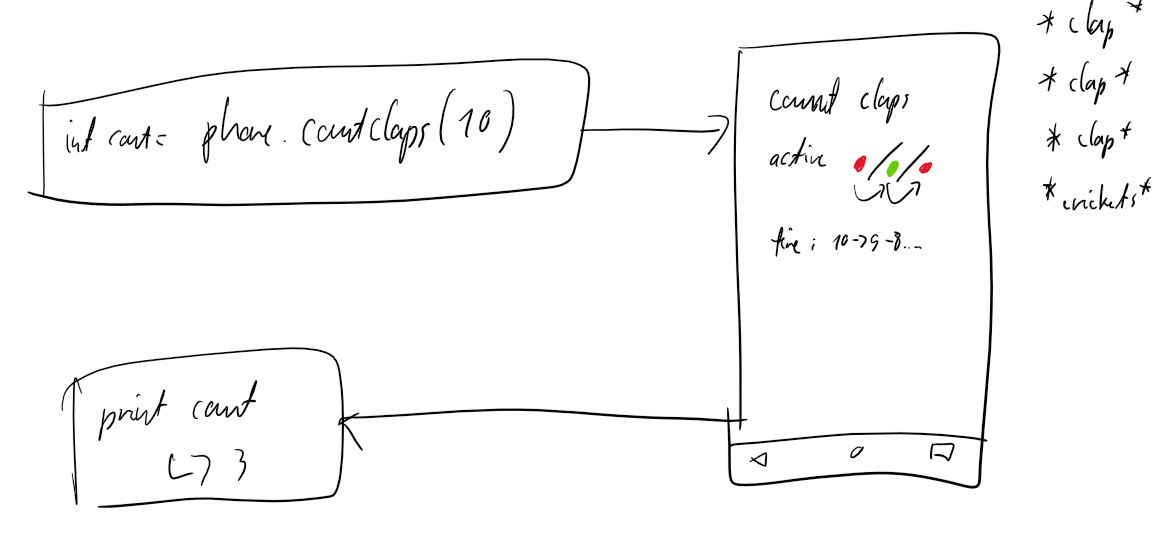
\includegraphics[width=.9\textwidth]{images/count_claps.png}
  \caption{Klatsch-Zähler}
  \label{fig:clap_count}
\end{figure}
% Vorgehen: \verb|num_of_spikes|
\\

\textbf{Dreh-Zähler}\\
Ein Nutzer möchte in einem bestimmten Zeitraum zählen wie oft das Smartphone gedreht wurde.

\section*{API}\label{sec:API}
Gelöst werden sollen die Aufgaben durch das Aufrufen der API.
Diese bietet die benötigten Funktionen an.
Die Aufrufe sind frei miteinander kombinierbar, so dass Aufgaben erweitert werden können.

\subsection*{Eingaben}

\textbf{Auslesen der accelerometer-Daten}\\
Ein User will den Wert der X, Y und Z Koordinaten des Smartphones wissen.
So kann er bspw. feststellen, ob das Smartphone gerade nach unten, oben oder horizontal bewegt wurde.
Kippbewegungen werden nicht detektiert.
\lstinputlisting[]{listings/api/acc.c}

\textbf{Lautstärkepegelmessung}\\
Ein User möchte den aktuellen Lautstärkepegel messen.
\lstinputlisting{listings/api/vol.c}

\textbf{Annäherungssensor-Messung}\\
Ein User möchte wissen, ob ein Objekt unmittelbar vor den Annäherungssensor steht.
Der Aufruf erfolgt folgendermaßen.
\lstinputlisting{listings/api/proxy.c}

\textbf{Amplituden-Spike-Messung mit Zeitraum}\\
Ein User möchte wissen, wie oft die Lautstärke innerhalb eines angegebenen Zeitraums t ein gewisses Limit überstiegen hat.
Der Aufruf könnte dabei folgendermaßen laufen.
\lstinputlisting{listings/api/numofspikes.c}


\textbf{Umdrehungsmessung mit Zeitraum}\\
Ein User möchte wissen, wie oft das Smartphone innerhalb eines angegebenen Zeitraums t gedreht wurde.
Der Aufruf sieht folgendermaßen aus.
\lstinputlisting{listings/api/numofspikes.c}


\subsection*{Ausgaben}\label{subsec:Ausgaben}

\textbf{Text-Ausgabe}\\
Um auf dem Smartphone einen beliebigen Text anzuzeigen.
Dies kann er zum Beispiel wie im folgenden Beispielcode machen.
\lstinputlisting[]{listings/api/display.c}

\textbf{LED leuchten lassen}\\
Ein User möchte eine "LED" auf dem Display ansteuern.
Dies kann er so machen.
\lstinputlisting[]{listings/api/led.c}

\textbf{LED toggeln}\\
Ein User möchte den Zustand einer LED auf dem Display auf "aus" stellen wenn Sie an war und auf "an" wenn Sie aus war.
Dies kann er so machen.
\lstinputlisting[]{listings/api/led.c}

\textbf{Vibrationsauslöser}\\
Ein Nutzer möchte das Smartphone für eine gewisse Zeitspanne vibrieren lassen.
\lstinputlisting[]{listings/api/vib.c}

\section*{Android Anwendung}
Für Ausgaben existiert eine Android Anwendung die verschiedene Interaktionsmöglichkeiten bereitstellt.
Das Userinterface wird in Grafik \ref{fig:android_ui} gezeigt.
\\
Bereit stehen eine LED bzw. ein Button, eine Textausgabezeile und eine Checkbox.
Der Button ist nicht drückbar.
Eine Eingabe ist nicht vorgesehen.
Er fungiert als Signal-LED die getoggelt werden kann.
\\
In der Textausgabe können beliebige Texte ausgegeben werden.
\\
Bei der checkbox kann der Haken gesetzt und wieder entfernt werden.
Nachdem der Zustand geändert wurde wird eine Antwort über den aktuellen Zustand der Checkbox zurückgegeben.


\section*{Softwareanforderungen}\label{sec:anforderungen}
Aus den unter \ref*{sec:API} genannten Funktionen ergeben sich die Anforderungen an das Framework.
\\
Es wird unterschieden in Funktionen die Sensordaten auslesen und Funktionen die Aktionen auf dem  auslösen.
\subsection*{Sensordaten-Funktionen}
Um das optimale Lernergebnis zu erhalten müssen Sensordaten responsiv vorliegen.
Je schneller Richtungs-, Helligkeits oder Lautstärkedaten vorliegen desto schneller kann im Programm drauf reagiert werden.
So können Experimente eher begriffen werden, da Auswirkungen in der Realität instantan Auswirkungen auf den vom Schüler geschriebenen Programmablauf haben.
Eine maximale Responszeit von ca. 20 ms ist hierfür zielführend.
\\
Beim Aufruf der Funktion wird kein Aufruf gestartet der das Smartphone anweist eine einzelne Sensormessung zu starten und den aktuell vorliegenden Sensorwert zurückzusenden.
Die Latenzen zwischen Smartphone und Bibliothek könnten je nach Verbindungsart, Bandbreite und Geräteanzahl im WLAN stark varrieren.
Das Smartphone muss in periodischen Abständen Sensordaten messen und senden. Die Sensorwerte werden dann zentral auf dem gleichen Rechner, auf dem auch die Bibliothek läuft zwischengespeichert.
So wird die mögliche Distanz zwischen Sender und Empfänger beschränkt auf den gleichen Rechner.
Sensordaten liegen immer zwischengespeichert vor.
Neue Daten werden beim Eintreffen der periodischen Aktualisierungen eingetragen.
Ein Funktionsaufruf der Sensordaten abfragt muss dann auf die zentral zwischengespeicherten Sensordaten zurückgreifen.
So wird der Responszeit erhöht und es liegt immer das aktuellste Sensor-Ergebnis im Zwischenspeicher vor.
Der Tätigkeitsbereich vom Smartphone umfasst jedoch nicht nur die Messung und Übermittlung der gemessenen Daten.

\subsection*{Auslösende Funktionen}
Die Anwendung auf dem Smartphone bietet ebenfalls verschiedene UI-Elemente welche aus der Ferne per Funktionsaufruf bedient werden.
Außerdem werden zeitlich beschränkte Messungen umgesetzt die auf Anfrage gestartet werden sollen.
Diese Art der Aufrufe benötigt keinen kontunierlichen Strom aus Werten, sondern wird einzeln aufgerufen und geben gegebenenfalls einzeln Werte zurück.
Der Fokus liegt bei diesen Anfragen nicht auf Responsivität, sondern auf Sicherheit des Aufrufs.
Bei dieser Art Aufruf werden Daten erst auf Anfrage generiert und dann, sofern vorgesehen, zurückgesendet.

\chapter{Architektur} \label{chap:architektur}
Der Aufbau des Frameworks besteht aus einer mobilen Anwendung für Android-Smartphones, Bibliothek in der Programmiersprache C und einer Middleware die den Austausch Koordiniert.
\\
Clientseitig erfolgen sämtliche Aufrufe die Sensordaten abgreifen oder Steueranfragen senden immer erst per UDP über die Middleware.
\\
Die Middleware sammelt, sobald sich eine Android-Anwendung bei ihr anmeldet, gewisse Sensordaten und speichert Sie intern zwischen, damit Sie schnell vorrätig vorliegen.
Die Speicherung erfolgt in einem seperaten Thread, der die letzten Zustände der Sensordaten hält.
Werden Sensordaten abgerufen werden Sie aus der Liste entfernt.
Sind noch keine Daten vorhanden, oder wird ein Sensor angefragt der im Smartphone nicht existent ist, wird ein Fehlercode zwischengespeichert.
Die Verfügbarkeit der jeweiligen Sensoren wird beim Start der Anwendung ermittelt.
\\
Steueraufrufe werden beim Aufruf über ein seperates Topic versandt.
Der Austausch erfolgt auf mehreren Topics, da manche Nachrichten, wie Steuerbefehle wie in \ref{subsec:Ausgaben} erwähnt, mit einem höheren QOS-Level versendet werden müssen als im Moment existente Sensordaten die nur eine kurzzeitige Relevanz besitzen und deren Zustellung nicht obligatorisch ist.
Auf diesem Topic werden Nachrichten mit der QOS von 2 versandt auf dem für reguläre Sensordaten mit einer QOS von 0.
% Todo: admin channel? Erster Aufbau auf admin channel mit anschließender negotiation auf welchen channeln gesendet werden soll. Wie hart aufziehen?
\begin{figure}[htbp]
  \centering
  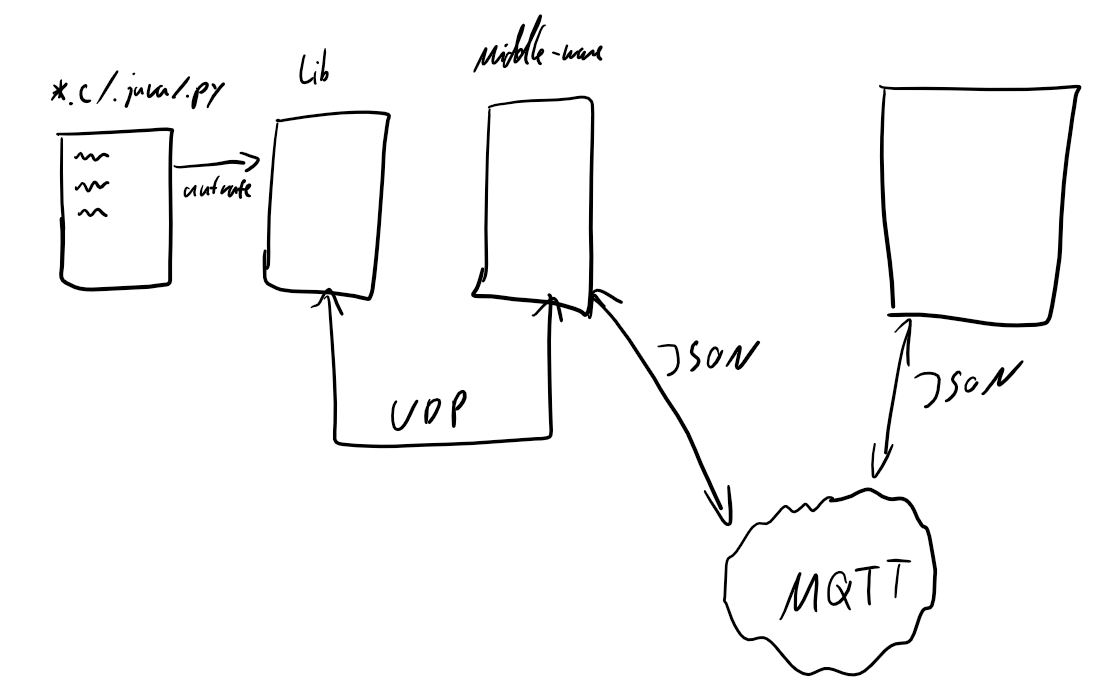
\includegraphics[width=.9\textwidth]{images/design.png}
  \caption{System-Aufbau}
  \label{fig:design}
\end{figure}


\section*{Android Anwendung}
Die Android-Anwendung läuft auf dem Smartphone des Anwenders.
Sie besteht aus einer Haupt-Activity deren außerlicher Aufbau in \ref{chap:intro} beschrieben ist. 
\\
In der Haupt-Activity wird ein Service gestartet und gebunden.
Der Service baut eine Verbindung zu einem MQTT Server auf.
Dort verbindet er sich den beiden Topics. 
Die Activity bindet beim Start den MQTT-Service ein.
Stellt ein Client über die Bibliothek auf einem Computer eine Anfrage wird dieser Aufruf, wie z.B. eine Ausgabe auf einem Textfeld an das Smartphones,  zuerst zur Middleware geleitet.
Diese leitet die Anfrage weiter an das Smartphone, dass dann den jeweiligen Befehl ausführt.
Dies beeinhaltet vor allem Ausgaben, sowie Eingaben die eine Nutzerinteraktion mit reduziertem Ergebnis.
Zum Beispiel alle Eingaben die etwas in einem angegebenen Zeitraum messen.
Falls ein Sensor angefragt wird der auf dem Smartphone nicht existiert wird eine Nachricht mit einer Fehlermeldung zurückgegeben.
\begin{figure}[htbp]
  \centering
  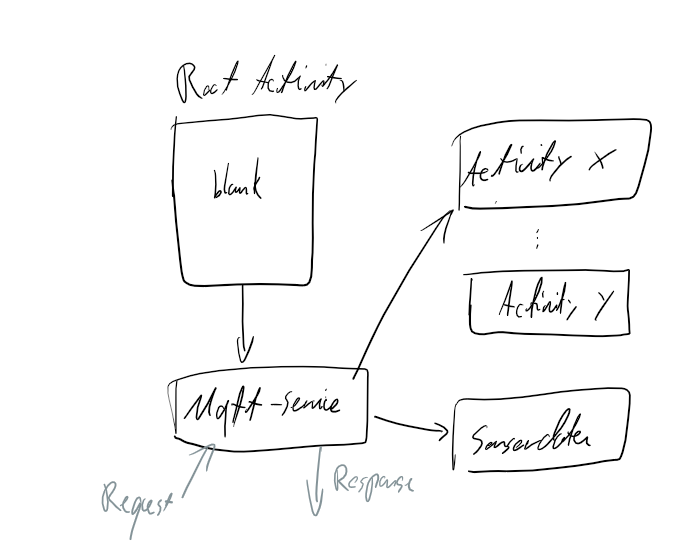
\includegraphics[width=.9\textwidth]{images/android_app.png}
  \caption{Android-App-Aufbau}
  \label{fig:android_app}
\end{figure}

\subsection*{Kommandos und Ausgaben}
Für die Ausgabe auf dem Smartphone sind verschiedene Kommandos definiert.
Diese sind der Tabelle \ref{tab:command_types} zu entnehmen.
\texttt{CMD-Kürzel} beschreibt die Notation des Kürzels mit dem eine Aktion ausgeführt werden kann.
Diese wird unter \texttt{Beschreibung} kurz zusammengefasst.
\texttt{return} gibt an, ob der Aufruf des Requests eine Antwort rücksendet und somit auch, ob ein Aufruf der Funktion in der Library blockiert oder nur sendet.
\begin{table}[htbp]
  \centering
  \begin{tabular}{|c|c|c|}
      \hline
      CMD-Kürzel & Beschreibung & return\\
      \hline
      textview & Setzt \texttt{value} als Text im Textvie & False \\
      button & Setzt Button auf value. Dies kann sein 
        \tabitem true : setzt die Farbe auf Grün \\
        \tabitem false : setzt die Farbe auf Rot \\
        \tabitem toggle : Kehrt die Farbe um \\
       & False \\
      \hline
  \end{tabular}
  \caption{Kommando-Kürzel mit Beschreibung}
  \label{tab:command_types}
\end{table}


\section*{Sensoren}
Smartphones beeinhalten verschiedene Sensoren die Daten über die Umgebung erfassen können.
In der Android Anwendung werden folgende Sensortypen verwendet:
\begin{itemize}
  \item Lineare Beschleunigungssensoren
  \item Microfon
  \item Annäherungssensor
  \item Gyroskop
\end{itemize}

\subsection*{Lineare Beschleunigungssensoren}
Beschleunigungssensoren messen die Beschleunigung in $m/s^2$ für die drei Bewegungsrichtungen: X-, Y- und Z-Achse in einem festgelegten Zeitraum.
Eine Übersicht über die Anordungen der drei Axen ist in Grafik \ref{fig:and_axes} zu sehen.
Die X-Achse verläuft horizontal durch das Display des Smartphones hindruch, die Y-Achse vertikal und die Z-Achse durchschneidet das Smartphone in die Tiefe.
\begin{figure}[htbp]
  \centering
  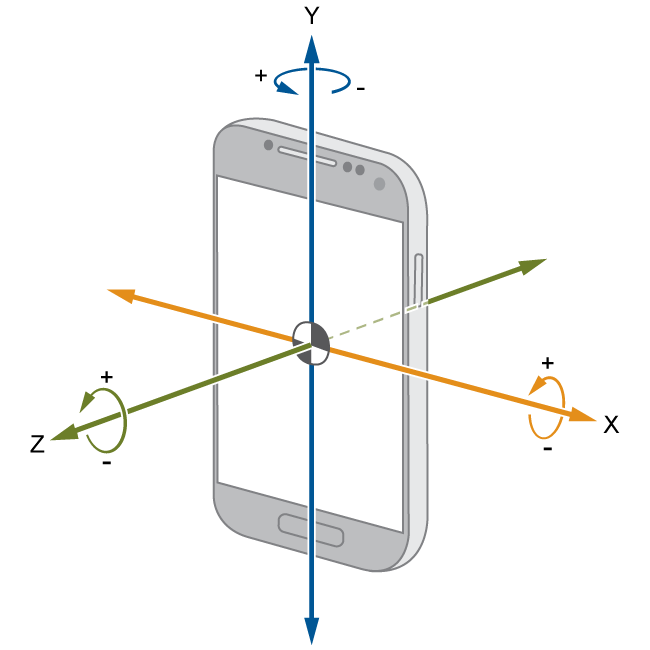
\includegraphics[width=.9\textwidth]{images/android_axes.png}
  \caption{Android-Koordinatensystem}
  \label{fig:and_axes}
\end{figure}

Die Beschleunigungsdaten werden dabei in einem festen Zeitraum gemessen.
Hierfür stehen vier Schnelligkeitsstufen in absteigender Frequenz bereit:
\begin{itemize}
  \item SENSOR\_DELAY\_FASTEST : Kein Verzögerung. Verwendet die Frequenz des Sensors.
  \item SENSOR\_DELAY\_GAME : Verzögerung um 1ms
  \item SENSOR\_DELAY\_UI : Verzögerung um 2ms
  \item SENSOR\_DELAY\_NORMAL : Verzögerung um 3ms
\end{itemize}
Die mit der jeweiligen Taktrate aufgenommenen Beschleunigungssensordaten umfassen jedoch auch die Ergbeschleunigung \texttt{g} in Höhe von $9.81 m/s^2$.
Diese muss für die bereinigten, realen Werte zuerst noch von den aufgenommenen Werten subtrahiert werden.
\\
Hierfür muss zuerst der Gleichanteil der Graviation mittels eines Tiefpassfilters von den gemessenen Werten isoliert werden.
\\
Der Algorithmus dafür ist folgendermaßen definiert:
\\
Für eine unendliche Folge an isolierten Gravitationswerten g und Beschleunigungssensor-Messwerten e mit index $n \in \mathbb{N} $ gilt:
\begin{equation}
  g_n = g_{n-1} \cdot \alpha + (1 - \alpha) \cdot e_n
\end{equation}
Die Konstante $\alpha$ wird dabei folgendermaßen berechnet:
\begin{equation}
  \alpha = t / (t + \Delta_t )
\end{equation}
$t$ ist dabei die Zeitkonstante des Tiefpass-Filters und $\Delta_t$ die Anpassungsrate.
\\
Die Berechnung des bereinigten Beschleunigungssensorwerts ist durch einen Hochpass definiert:
\\\\
Für eine unendliche Folge an ereinigten Beschleunigungssensor-Messwerte l, isolierten Gravitationswerten g und Beschleunigungssensor-Messwerten e  mit index $n \in \mathbb{N}$ gilt:
\begin{equation}
  l_n = e_n - g_n
\end{equation}
Die Graviation könnte auch unter Zuhilfenahme des Gyroskops isoliert werden.
Die wirkenden Kräfte auf die drei Achsen könnten je nach Neigung einzeln bemessen werden.
Hierfür müsste die Masse des Smartphones jedoch bekannt und gleich verteilt sein.
Deshalb wird hierfür auf die Pragmatische Hochpass-Tiefpass-Lösung zurückgegriffen.


\subsection*{Angaben für die Nachrichtenformate}
Alle Sensordaten besitzen ein festgelegtes Kürzel zur Standardisierung des Nachrichtenverkehrs.
Sie dienen vor allem der Adressierung der jeweiligen Daten in der Middleware und in der Library.
\\
Die Sensortyp Kürzel sind in Tabelle \ref{tab:sensor_types} zu finden. 
\begin{table}[htbp]
  \centering
  \begin{tabular}{|c|c|c}
      \hline
      TYPE-Kürzel & Beschreibung \\
      \hline
      accell\_x & Beschleunigungssensor für die X-Richtung \\
      \hline
      accell\_y & Beschleunigungssensor für die Y-Richtung \\
      \hline
      accell\_z & Beschleunigungssensor für die Z-Richtung \\
      \hline

  \end{tabular}
  \caption{Sensor-Kürzel mit Beschreibung}
  \label{tab:sensor_types}
\end{table}



\chapter*{Nachrichtenformate}
Damit der gesamte Funktionsablauf des Frameworks korrekt funktioniert müssen Nachrichten zwischen den einzelenen Komponenten ausgetauscht werden.
Hierfür wird ein Format definiert dass die in Kapitel \ref{sec:anforderungen} erwähnten Anforderungen sowohl auf Library-, Middleware-, und Smartphone-Seite umsetzt.

Die Nachrichten werden im JSON-Format übertragen.
Jede Nachricht beeinhaltet mindestens die Angabe eines Nachrichtenformat-Typs.
Für die Aufrufe wurden folgende Nachrichtenformate definiert:
\begin{enumerate}
  \item sensor\_request
  \item sensor\_update\_request
  \item rpc\_request
  \item rpc\_response
\end{enumerate}
Die Nachrichtenformate werden als Vorlagen in einer zentralen Datei abgelegt.
Diese werden in der Library, Middleware und auf dem Smartphone eingelesen, damit Sie nur einer Stelle definiert werden müssen, wie in \ref*{fig:all_json} dargestellt.
Neben den Nachrichtenformaten werden hier auch weitere Konfigurations-Konstanten wie Commands für rpc\_requests, Namen der Sensordaten und Namen der MQTT Topics spezifiziert spezifiziert.


\begin{figure}[htbp]
  \centering
  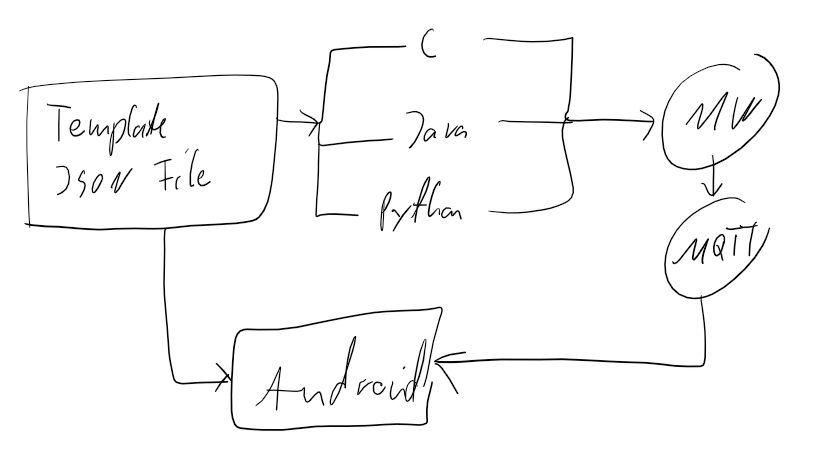
\includegraphics[width=.9\textwidth]{images/all_json.png}
  \caption{Zentrale Konfigurationsdatei}
  \label{fig:all_json}
\end{figure}


\textbf{sensor\_requests} werden vom Endanwender-PC per UDP an die Middleware gesendet.
Sie beeinhalten neben dem Typ das Feld \texttt{sensor\_type}.
Dieses definiert den Sensortyp für den eine Anfrage generiert wurde.
Eine Übersicht ist in Listing \href{lst:sensor_request} zu finden.
\\
Im Listing wurde der Platzhalter \texttt{TYPE} für alle möglichen Sensortypen angegeben.
Eine vollständige Aufschlüsselung ist in Tabelle \ref{tab:sensor_types} zu finden.
\lstinputlisting[label={lst:sensor_request}, caption={sensor\_request}, captionpos=b]{listings/messages/sensor_request.json}

\textbf{sensor\_update\_requests} werden von Smartphone über MQTT an die Middleware versandt.
Sie umfassen ebenfalls wie \texttt{sensor\_requests} das Feld \texttt{sensor\_type}, jedoch zusätzlich auch das Feld \texttt{value} in dem der gemessene Sensorwert gespeichert wird.
Dieser wird von der Middleware in eine interne Datenstruktur eingetragen.

\textbf{rpc\_requests} werden vom Endanwender-PC per UDP an die Middleware gesendet.
Sie lösen Aktionen auf dem Smartphone aus wie zum Beispiel das anschalten der LED, oder das Starten von Messungen.
Sie werden von der Middleware per MQTT an das Smartphone weitergereicht.
Die Übermittlung erfolgt jedoch über ein seperates Topic mit einem Quality of Service Wert von 2 um eine garantierte Übertragung zu gewährleisten.
Das Smartphone hat dieses TOPIC ebenfalls mit einer QOS von 2 abboniert.
eine Liste der Tabelle \ref{tab:command_types} zu entnehmen.




rpc\_requests und response beeinhalten außerdem mindestens ein \texttt{command}-Feld und ein \texttt{value}-Feld.

Nachfolgendes Listing zeigt beispielsweise den Aufruf die LED einzusschalten.

\lstinputlisting[]{listings/messages/led.json}
Folgende Nachricht beschreibt beispielsweise den übermittelten Sensorwert des accelerometers.
\lstinputlisting{listings/messages/accell.json}

\section*{Nachrichtenablauf}

Der Nachrichtenablauf ist in Grafik \ref*{fig:message flow} dargestellt.
\\
Grau dargestellt ist hier die periodische aktualisierung der Sensordaten durch sensor\_update\_requests.
Diese werden mit einer auf dem Smartphone definierten Taktung an die Middleware übertragen
Die Middleware trägt die neuen Daten dann in der internen Datenbank ein.
\\
Grün dargestellt ist der Ablauf eines sensor\_requests.
Aus der Library heraus werden sensor\_requests gesendet.
Die Middleware, die die aktuellen Sensorwerte vorhält sendet dann als Antwort den Sensorwert als einzelnen Wert, also nicht im JSON-Format zurück.
\\
Blau dargestellt ist ein rpc\_request, dass ein Command auf dem Smartphone ausführt, dass keinen Rückgabewert zurückliefert. Änlich wie bei sensor\_update\_requests handelt es sich hier um fire-and-forget-requests.
\\
Lila dargestellt sind rpc\_requests die ein Command ausführen dass einen Rückgabewert erwartet, wie es beispielsweise bei zeitlich getakteten Messungen der Fall ist. 
In diesem Fall wird eine rpc\_response-Nachricht mit versendet.

\begin{figure}[htbp]
  \centering
  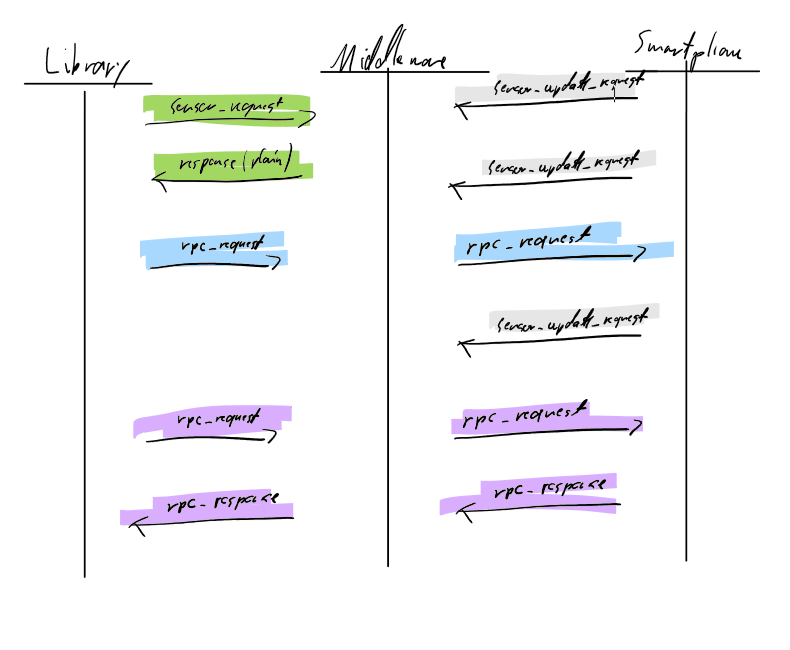
\includegraphics[width=.9\textwidth]{images/message_flow.png}
  \caption{Nachrichtenablauf}
  \label{fig:message flow}
\end{figure}

\section*{Verwendete Technologien}
In diesem Kapitel werden die Technologien und Protokolle beschrieben die beim Nachrichtenaustausch zwischen Library, Middleware und Smartphone zum Einsatz kommen.
\\
Der Fokus liegt auf Serialisierung und Transport.
Da im gesamten Prozess zwischen den drei Einheiten unterschiedliche Programmiersprachen auf verschiedenen Plattformen zum Einsatz kommen müssen sämtliche Protokolle und Notationen von möglichst vielen Programmiersprachen unterstztützt werden.
\\
Beim Transport liegt die Anforderung vor allem auf einer schnellen Ausführung, da sich Sensordaten schnell ändern und ein Lerneffekt am Besten eintritt wenn keine hohen Latenzen bei der Übertragung auftreten.

\subsection*{JSON}
JSON ist eine Abkürzung für JavaScript Object Notation.
Es handelt sich um ein Nachrichten-Austausch-Format \cite{json}
\\\\
Der Aufbau ist minimalistisch. Objekte können mit Schlüssel-Wert-Paaren serialisiert werden.
Auch Arrays können eingesetzt werden.
Durch den einfachen Aufbau werden für eine Nachricht auch nicht viele Ressourcen benötigt.
Gerade bei der Übertragung von Sensordaten ist ein schneller Datenaustausch sehr positiv.
\\
JSON wird außerdem von vielen Programmiersprachen wie Python und Java nativ unterstützt.
Da die Bibliotheken programmiersprachenunabhäng bereitgestellt werden sollen bietet sich JSON als gemeinsame Notation hervorrangend an.
Da es in C keinen eingebauten JSON Parser gibt wird hier auf den cJSON \cite{cjson} zurückgegriffen.

\subsection*{MQTT}
MQTT steht für Message Queuing Telemetry Transport und ist ein Client-Server Protokoll das auf TPC basiert.
Es kommt häufig mei Machine-to-Machine Interaktionen zum Einsatz.
Dies umfasst Lösungen im IoT-, Smarthome und Automatisierungstechnik-Bereich.
Durch den platzsparenden Header von 2 Bytes und einer maximalen Nachrichtengröße von ca. 260 MB ist es gleichzeitig ein leichtgewichtiges jedoch auch flexibles Protokoll zum Nachrichtenaustausch.
\\
Für den Nachrichtenaustausch registrieren sich Clients an einem Broker, dem MQTT-Server, an ein oder mehrere Topics.
Auf diesen Topics können dann Nachrichten gesendet und empfangen werden.
Topics können hierarchisch geschichtet werden.
Subtopics können dann pro ebene oder rekursiv für alle Subtopics abboniert werden.
Dieses Feature ist jedoch für die Entwicklung nicht weiter von Belang.
Nachrichten werden von Clients an den Broker gesendet.
Dieser hält den Nachrichteninhalt intern für das jeweilige Topic.
\\
Alle Clients besitzen einen Identifier, so dass empfangene Nachrichten zurückgeführt werden können.
Somit sind auch Topic-Interne Filter möglich nur Nachrichten von bestimmten Clients zu empfangen.
\\
Nachrichten können mit einer Quality of Service (QoS), einer Übertragungsgüte, übertragen werden.
Insgesamt gibt es drei Stufen: 0, 1 und 2.
Je höher die QoS-Stufe desto höher die Latenz der Übertragung.
\\
Bei einer QoS von 0 werden Daten einfach übertragen ohne sicherzugehen, dass die Nachricht auch wirklich beim Broker ankommt. 
Bei QoS 1 wird eine Nachricht so lange auf einem Topic gesendet bis der Broker den Empfang einmal bestätigt.
Es kann jedoch auch passieren, dass der Broker die Nachricht mehrmals empfängt und nur einmal bestätigt.
Bei QoS 2 wird die Nachricht einmal an den Broker gesendet.
Dieser muss dann den Empfang der Nachricht einmal bestätigen.
Erst dann gilt die Nachricht als Empfangen.
\\
Damit die verlangte Güte sichergestellt wird müssen Sender und Empfänger mit der gleichen Güte senden bzw. ein Topic mit der gleichen Güte-Stufe abbonieren.
Wird ein Topic mit einer geringeren Güte abboniert als die Güte der publizierten Nachricht wird die Nachricht mit der Güte des Abbonenten übertragen.
Wenn eine Nachricht mit geringerer Güte auf einem Topic publiziert wurde als dieses Topic abboniert wurde wird die Übertragung mit der Güte-Stufe des publizierenden Clients übertragen.

\subsection*{UDP}
UDP ist ein verbindungsloses Netzwerkprotokoll, dass auf der Transportschicht des TCP/IP-Stack zum Einsatz kommt.



\chapter*{Fazit}


% Listen wenn überhaupt ans Ende und nicht an den Anfang.
% Meist ist das aber unnötig.
% \listoffigures % Liste der Abbildungen 
% \listoftables % Liste der Tabellen
% \newpage

\bibliographystyle{plain} % Literaturverzeichnis
\begin{btSect}{thesis} % mit bibtopic Quellen trennen
\addcontentsline{toc}{chapter}{Literaturverzeichnis und Online-Quellen}
\section*{Literaturverzeichnis}
\btPrintCited
\end{btSect}
\begin{btSect}{online}
\section*{Online-Quellen}
\btPrintCited
\end{btSect}
% dann mit "bibtex thesis1" und "bibtex thesis2" arbeiten

\end{document}
;;; Local Variables:
;;; ispell-local-dictionary: "de_DE-neu"
;;; End:


